\documentclass[tikz,border=2pt]{standalone}
\usepackage{amsmath,amssymb}
\usepackage{tikz}

\begin{document}
% Ordering cycle: pencils, y = 6000 per order, D = 100 per day, so t0 = y/D = 60 days between
% consecutive orders and D/y = 1/60 orders per day.
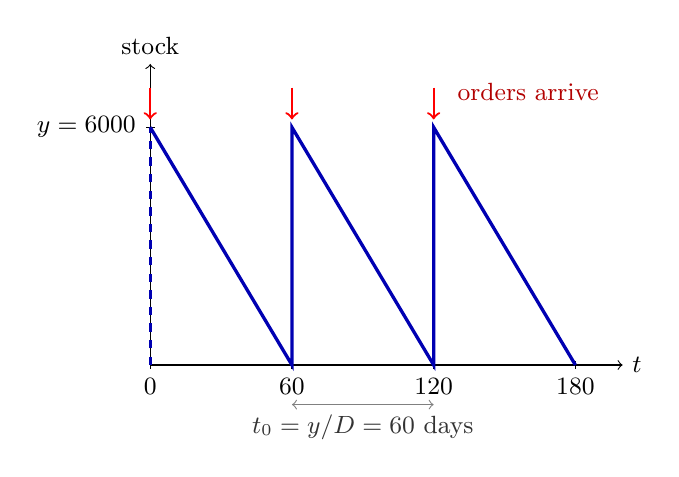
\begin{tikzpicture}[every node/.style={font=\small}, x=0.03cm, y=0.0005cm]
	\draw[->] (0,0) -- (200,0) node[right] {$t$};
	\draw[->] (0,0) -- (0,7600) node[above] {stock};
	\foreach \t in {0,60,120,180} {\draw (\t,100) -- (\t,-100) node[below] {$\t$};}
	\draw (2,6000) -- (-2,6000) node[left] {$y=6000$};
	\draw[blue!70!black, very thick] (0,6000) -- (60,0) -- (60,6000) -- (120,0) -- (120,6000) -- (180,0);
	\draw[blue!70!black, very thick, dashed] (0,0) -- (0,6000);
	\foreach \t in {0,60,120} {\draw[->, red, thick] (\t,7000) -- (\t,6200);}
	\node[red!70!black, anchor=west] at (126,6900) {orders arrive};
	\draw[<->, gray] (60,-1000) -- (120,-1000) node[midway, below, text=gray!40!black] {$t_0=y/D=60$ days};
\end{tikzpicture}
\end{document}
